\documentclass[cjk,dvipdfmx,10pt,compress,%
hyperref={bookmarks=true,bookmarksnumbered=true,bookmarksopen=false,%
colorlinks=false,%
pdftitle={第 117 回 関西 Debian 勉強会},%
pdfauthor={倉敷・のがた・佐々木・かわだ・おおつき},%
%pdfinstitute={関西 Debian 勉強会},%
pdfsubject={資料},%
}]{beamer}

\title{第 117 回 関西 Debian 勉強会}
\subtitle{$\sim$発表資料$\sim$}
\author[かわだ てつたろう]{{\large\bf 倉敷・のがた・佐々木・かわだ・おおつき}}
\institute[Debian JP]{{\normalsize\tt 関西 Debian 勉強会}}
\date{{\small 2016 年 12 月 25 日}}

%\usepackage{amsmath}
%\usepackage{amssymb}
\usepackage{graphicx}
\usepackage{moreverb}
\usepackage[varg]{txfonts}
\AtBeginDvi{\special{pdf:tounicode EUC-UCS2}}
\usetheme{Kyoto}
\def\museincludegraphics{%
  \begingroup
  \catcode`\|=0
  \catcode`\\=12
  \catcode`\#=12
  \includegraphics[width=0.9\textwidth]}
%\renewcommand{\familydefault}{\sfdefault}
%\renewcommand{\kanjifamilydefault}{\sfdefault}
\begin{document}
\settitleslide
\begin{frame}
\titlepage
\end{frame}
\setdefaultslide

\begin{frame}[fragile]
  \frametitle{Disclaimer}
  \begin{itemize}
  \item 疑問、質問、ツッコミ、茶々、\alert{大歓迎}
  \item その場でインタラクティブにどうぞ
  \item ハッシュタグ \#kansaidebian
  \end{itemize}
\end{frame}

\begin{frame}[fragile]
\frametitle{Agenda}

\tableofcontents

\end{frame}

\section{最近の Debian 関係のイベント}

\takahashi[40]{最近の Debian\\関係のイベント}

\begin{frame}[fragile]
  \frametitle{第115回関西Debian勉強会}
  \begin{itemize}
  \item 日時: 10月23日(日)
  \item 場所: 港区民センター
  \end{itemize}
  \begin{block}{内容}
    \begin{itemize}
    \item sbuild と debci を触ってみた
    \end{itemize}
  \end{block}
\end{frame}

\begin{frame}[fragile]
  \frametitle{第116回関西Debian勉強会@KOF}
  \begin{itemize}
  \item 日時: 11月12日(土)
  \item 場所: 大阪南港 ATC
  \end{itemize}
  \begin{block}{内容}
    \begin{itemize}
    \item Debian updates
    \item ブース展示
    \end{itemize}
  \end{block}
\end{frame}

\begin{frame}[fragile]
  \frametitle{第145回東京エリアDebian勉強会 OSC 2016 Tokyo/Fall 出張}
  \begin{itemize}
  \item 日時: 11月5日(土)、6日(日)
  \item 場所: 明星大学 日野キャンパス
  \end{itemize}
  \begin{block}{内容}
    \begin{itemize}
    \item Debian updates
    \item ブース展示
    \end{itemize}
  \end{block}
\end{frame}

\begin{frame}[fragile]
  \frametitle{第146回東京エリアDebian勉強会}
  \begin{itemize}
  \item 日時: 11月19日(土)
  \item 場所: 株式会社 朝日ネット
  \end{itemize}
  \begin{block}{内容}
    \begin{itemize}
    \item 「dh\_strip\_nondeterminism」
    \end{itemize}
  \end{block}
\end{frame}

\begin{frame}[fragile]
  \frametitle{Mini Debian Conference Japan 2016}
  \begin{itemize}
  \item 日時: 12月10日(土)
  \item 場所: サイボウズ株式会社
  \end{itemize}
\end{frame}

\begin{frame}[fragile]
  \frametitle{Debian Project}
  \begin{itemize}
  \item Release update: Debian 9 'Stretch'
  \item Accepted global 6.5.5-0.1 (source amd64) into experimental
  \end{itemize}
\end{frame}

\takahashi[50]{そんな\\こんなで}
\takahashi[120]{次}

\takahashi[50]{事前課題}

\begin{frame}[fragile]
  \frametitle{事前課題}
  \begin{block}{今回の事前課題}
    \begin{description}
    \item[事前課題1]
      2016 年はどうでしたか?
    \item[事前課題2]
      2017 年の目標は?
    \end{description}
  \end{block}
\end{frame}

\takahashi[50]{事前課題\\発表}

\begin{frame}
  \frametitle{ t3rkwd }
  \begin{enumerate}
  \item なぜか関西のイベントに参加できない年でした。
  \item まずは Stretch リリースに向けて何か。
  \end{enumerate}
\end{frame}

\begin{frame}
  \frametitle{ Katsuki Kobayashi }
  \begin{enumerate}
  \item 勉強会への参加率はそこそこ頑張りましたが、結局Debian自体の勉強はあまりし
    なかったかなぁ……と。
  \item Debianになにかしらcontributeしていきたい。
    (まずはStretchになにかしら貢献して勉強会で発表?)
  \end{enumerate}
\end{frame}

\begin{frame}
  \frametitle{ uwabami }
  \begin{enumerate}
  \item イベント関連に余り貢献できなかったのが残念でした。
  \item いよいよ Stretch がリリースされますね。
  \end{enumerate}
\end{frame}

\begin{frame}
  \frametitle{ ipv6waterstar }
  \begin{enumerate}
  \item いろんな意味で、激動の一年かな?
  \item 海外旅行、パッケージを作ってみる。
  \end{enumerate}
\end{frame}

\begin{frame}
  \frametitle{ Yosuke OTSUKI }
  \begin{enumerate}
  \item あんまり OSS  の活動できなかった
  \item Debian の管理者になる。モントリオール行きたい。
  \end{enumerate}
\end{frame}

\takahashi[50]{そんな\\こんなで}
\takahashi[120]{次}

\section{2016年の振り返りと2017年の企画}
\takahashi[30]{2016年の振り返りと2017年の企画\\by\\Debian JP}

\takahashi[50]{2016年を\\振り返って}
\begin{frame}
  \frametitle{今年のお題一覧}
  {\footnotesize
    \vspace{1em}
    \begin{table}
      \centering
    \begin{tabular}{|l|c|l|p{26em}|}
      \hline
      開催年月  & 参加 & 内容 \\
      \hline
        2016年1月 & 12    & \color<2->[rgb]{1,0,0}{GNUHurdのインストールしてみた。と、Xサーバの立ち上げに挑戦} \\
                  &       & \color<2->[rgb]{1,0,0}{VyOSを入れてAPを構築してみた。}\\
      \hline
        2016年2月 & 10    & 勉強会資料の歩き方 \\
                  &       & \color<2->[rgb]{1,0,0}{周回遅れでDocker触ってみた} \\
      \hline
        2016年3月 & 10    & \color<2->[rgb]{1,0,0}{systemd に浸かってみる} \\
      \hline
        2016年4月 & 9     & \color<2->[rgb]{1,0,0}{OpenFOAM による数値流体解析} \\
      \hline
        2016年5月 & 3     & ライトニングトーク \& もくもくの会  \\
      \hline
        2016年6月 & 11    & \color<3->[rgb]{0,1,0}{Debian パッケージング道場} \\
      \hline
        2016年7月 &       & \color<4->[rgb]{0,0,1}{OSC 2016 @ Kyoto} \\
      \hline
        2016年8月 & 9     & ライトニングトーク \& もくもくの会 \\
      \hline
        2016年9月 & 5     & \color<3->[rgb]{0,1,0}{初心者が初めてパッケージをつくってみた} \\
                  &       & \color<2->[rgb]{1,0,0}{Let's Encryptのススメ} \\
      \hline
        2016年10月& 7     & \color<2->[rgb]{1,0,0}{sbuild と debci を触ってみた} \\
      \hline
        2016年11月&       & \color<4->[rgb]{0,0,1}{KOF 2016} \\
      \hline
        2016年12月& 7     & 2016年の振り返りと2017年の企画, 忘年会 \\
      \hline
    \end{tabular}
    \end{table}
  }
\end{frame}

\begin{frame}
  \frametitle{2016年の参加状況}
  \centering
  関西の参加人数推移(参加人数と6ヶ月移動平均、アンケート回答人数)
  \begin{figure}[h]
    \begin{center}
      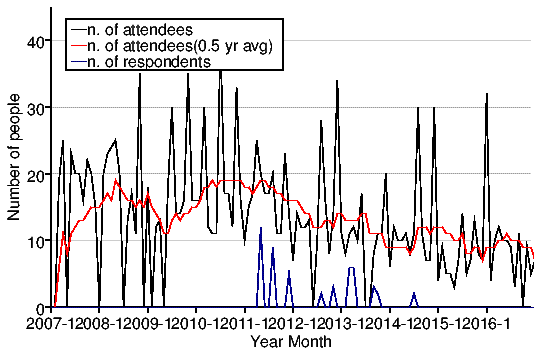
\includegraphics[width=.6\hsize]{image201612/memberanalysis/kansai.png}
    \end{center}
  \end{figure}
\end{frame}

\begin{frame}
  \frametitle{今年のイベント/お題}
  \begin{itemize}
  \item もくもくの会
  \item \color[rgb]{1,0,0}{セッション}
    \begin{itemize}
    \item GNUHurdのインストールしてみた, VyOSを入れてAPを構築してみた,
      周回遅れでDocker触ってみた, systemd に浸かってみる, OpenFOAM による数値流体解析,
      Let's Encryptのススメ, sbuild と debci を触ってみた
    \end{itemize}
  \item \color[rgb]{0,0,1}{イベント}
    \begin{itemize}
    \item OSC 2016 Kansai@Kyoto, KOF 2016
    \end{itemize}
  \end{itemize}
\end{frame}

\begin{frame}
  \frametitle{定例ネタ(パッケージ作成, バグ報告など)}
  \begin{exampleblock}{背景・目的}
    {\small{
        2007年度から関西でも Debian 勉強会を始動しています。
        \alert{短期的な目標は、Debian Developer(Debian開発者,以下DD) を増やすことです。}
        東京ではDebian勉強会が開催されてきましたが、一方の関西は、東京にくらべて DD の数が少ないです。 関西 Debian 勉強会は、DD と出会って GPG Key Sign をするチャンスを提供します。 また、勉強会を行うことを通して、Debian に関する知識を共有します。}}
    \vskip.5em
    \hspace*\fill{\small--- http://wiki.debian.org/KansaiDebianMeeting}
  \end{exampleblock}
  \begin{itemize}
  \item パッケージング道場
  \item 初心者が初めてパッケージをつくってみた
  \end{itemize}
\end{frame}

\begin{frame}
  \frametitle{運営}
  \begin{itemize}
  \item 運営フロー
  \item ネタの見直し
  \item リソース不足
  \end{itemize}
\end{frame}

\begin{frame}
  \frametitle{イベント}
  \begin{itemize}
  \item 定例は以下の通り
    \begin{description}
    \item[OSC Kansai@Kyoto] \mbox{~}\\
      来年も8月
    \item[KOF 2017] \mbox{~}\\
      来年も11月
    \item[OSC Kansai@Osaka 2018] \mbox{~}\\
     2018 年は参加したい。
    \end{description}
  \end{itemize}
\end{frame}

\takahashi[50]{2016年の企画}

\begin{frame}
  \frametitle{2016年の企画}
  \begin{itemize}
  \item
  \end{itemize}
\end{frame}

\begin{frame}
  \frametitle{2017年の開催日}
  \begin{itemize}
  \begin{tiny}
  \item 1月29日({\color{red}日}) 港区区民センター 楓 \\
   openSUSE / LILO\&東海道らぐ 合同開催
  \item 2月26日({\color{red}日}) 福島 区民センター 304 \\
   パッケージング (kobayashi さん) \& Bug squashing party ?
  \item 3月26日({\color{red}日}) 福島 区民センター 304 \\
      10 周年記念
  \item 4月23日({\color{red}日}) 福島 区民センター 304 \\
   リリースパーティ ? \\
   リリースなければ、CMake (otsuki)
  \item 5月28日({\color{red}日}) 福島 区民センター 304 \\
   リリースパーティ ? \\
   リリースなければ、CMake (otsuki)
  \item 6 月 パッケージング道場
  \item 7 月 GNU PG \& Ybi key (sasaki)
  \item 8 月 OSC Kyoto ?
  \item 9 月
  \item 10 月
  \item 11 月 KOF
  \item 12 月 忘年会
  \end{tiny}
  \end{itemize}
\end{frame}

\takahashi[50]{そんな\\こんなで}
\takahashi[50]{来年も頑張りましょう}

\takahashi[120]{次}

\section{今後の予定}
\begin{frame}[fragile]
\frametitle{今後の予定}

\begin{block}{第118回関西Debian勉強会}
  \begin{itemize}
  \item 日時: 1月29日(日)
  \item 場所: 港区民センター
  \item 内容: openSUSE / LILO\&東海道らぐ 合同開催
  \end{itemize}
\end{block}

\begin{block}{第147回東京エリアDebian勉強会}
  \begin{itemize}
  \item 日時: 1月21日(土)
  \item 場所: ?
  \end{itemize}
\end{block}

\end{frame}

\takahashi[50]{  }

\end{document}
%%% Local Variables:
%%% mode: japanese-latex
%%% TeX-master: t
%%% End:
